\documentclass{article}
\title{Ant Colony Optimisation for the Travelling Salesman Problem}
\author{Dylan Galea}

\usepackage{cite}
\usepackage{amsmath}
\usepackage{amsthm}
\usepackage{amssymb}
\usepackage{physics}
\usepackage{tikz}
\usetikzlibrary{arrows.meta,automata,positioning}

\newtheorem{theorem}{Theorem}[subsection]
\newtheorem{definition}{Definition}[subsection]
\newtheorem{lemma}[definition]{Lemma}
\newtheorem*{remark}{Remark}
\newtheorem{example}[definition]{Example}

\begin{document}
\maketitle
\newpage
\tableofcontents
\newpage
\section{Introduction}
Before defining the Travelling Salesman Problem and proving properties about it, a number of concepts must first be defined. Therefore, what follows is a sub-section that introduces a number of graph theoretic concepts which are required for the Travelling Salesman Problem.
\subsection{Some Graph Theory}
Graph theory is the study of the structure called a graph. A graph can be defined formally as shown in definition \ref{Graph} below.
\begin{definition}[Graph]
\label{Graph}
A graph G is a pair (V,E) were V is any finite set called the set of vertices of G, and E $\subseteq$ \{$\{u,v\}$ $:$ u,v $\in$ V and u $\neq$ v\} is called the set of edges of G {\normalfont{\cite{black_tanenbaum_2017}}}. A graph G defined by the pair (V,E) is denoted by G(V,E).
\end{definition}
A graph defined as in definition \ref{Graph} is called an undirected graph. There is also the concept of a directed graph were E $\subseteq$ \{(u,v) $:$ u,v $\in$ V and u $\neq$ v\} \cite{black_tanenbaum_2017}. However, in this thesis it can be assumed that any graph that will be considered is undirected unless otherwise stated. It can also be assumed that there are no edges between same vertices unless otherwise stated.
\begin{definition}
\label{adjacent}
Given a graph G(V,E), $\forall$ u,v $\in$ V, u and v are said to be adjacent if \{$u,v\}$ $\in$ E. \normalfont{\cite{weisstein_2018_3}}
\end{definition}
Any graph G(V,E) can also be illustrated pictorially by representing the vertices of G using dots, and by representing the edges of G using lines between adjacent vertices. Example \ref{Example 1} below depicts how a graph can be represented pictorially.
\begin{example}
\label{Example 1}
Consider the graph G(V,E) such that  V=\{$v_1, v_2, v_3, v_4\}$ and E = \{$\{v_1, v_2\}, \{v_2,v_3\}, \{v_3,v_4\}, \{v_4,v_1\}\}$.\\Then G can be represented pictorially as :\\

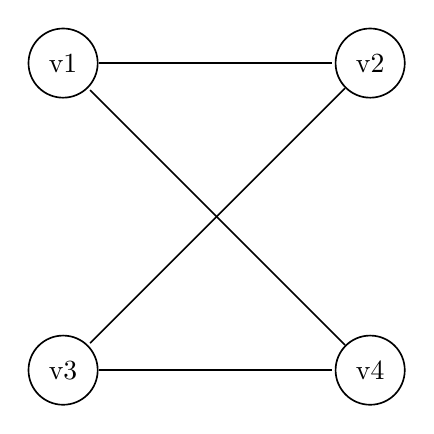
\begin{tikzpicture}[
    > = , % arrow head style
    shorten > = 1pt, % don't touch arrow head to node
    auto,
    node distance = 3cm, % distance between nodes
    semithick % line style
    ]

    \tikzset{every state}=[
    draw = black,
    thick,
    fill = black,
    minimum size = 1mm
    ]

    \node[state] (v1) {v1};
    \node[state] (v2) [right=of v1] {v2};
    \node[state] (v3) [below =of v1] {v3};
    \node[state] (v4) [below =of v2] {v4};
  
    \path[->] (v1) edge  node[]{}(v2);
    \path[->] (v2) edge  node[]{} (v3);
    \path[->] (v3) edge  node[]{}(v4);
    \path[->] (v4) edge  node[]{}(v1);
\end{tikzpicture}
\end{example}
There are many other examples of graphs, one of them being the complete graph on $\mathit{n}$ vertices.
\begin{definition}[Complete Graph]
\label{Complete Graph}
A graph G(V,E) is said to be complete if $\forall$ v,w $\in$ V v $\neq$ w, v is adjacent to w. The complete graph on n vertices is denoted by $K_n$. \normalfont{\cite{complete_graphs}}
\end{definition}
Given any graph G(V,E) one can also define the concept of a path.
\begin{definition}[Path]
\label{Path}
Given a graph G(V,E), a path in G joining the vertices u,v $\in$ V is a sequence of vertices u = $u_1$, $u_2$, ...,$u_n$ = v in which no vertex is repeated and, $\forall$ $u_i$,$u_{i+1}$ i $\in$ [n-1], \{$u_i,u_{i+1}\}$ $\in$ E. \normalfont{\cite{thompson}  }
\end{definition}
Using definition \ref{Path}, the concept of a cycle can now be defined.
\begin{definition}
\label{cycle}
\end{definition}
Example \ref{example3} below illustrates definitions \ref{Complete Graph}, \ref{Path}, \ref{cycle} above.
\begin{example}
\label{example3}
\end{example} 
\newpage
\section{The Travelling Salesman Problem}
\subsection{Heuristics}
\section{The Ant Colony Algorithm}
\newpage
\section{Experimental Data}
\newpage
\section{Conclusion}
\newpage
\bibliography{bibliography}
\bibliographystyle{IEEEtran}
\end{document}